\subsection{Diagnosing and revising the restricted point geometry}
\label{sec:he0435-geometry-revision}

The failed Gaia experiment in Section~\ref{sec:he0435-gaia} now supplies
development data, rather than another validation opportunity. Its discrepancy
is largely present before the Gaia comparison: the frozen conventional model
misses the NIC2 coordinates used for its fit by 3.0913~mas coordinate RMS,
whereas Gaia and those NIC2 measurements differ by 1.2469~mas RMS. Exact
gnomonic projection changes the old comparison by at most 0.00322~mas.
Fitting a global rotation and scale reduces the Gaia residual only from
3.2556 to 3.2393~mas. The image labels, east/north convention, common-A
covariance and original stationary-ray residuals therefore do not explain
the principal failure.

Nor does more optimization within the same declared family resolve it.
Using all nine original parameters, the unchanged Gaia covariance and no
delay or centroid penalties gives a local best quadratic residual of
1559.08, with 2.9861~mas coordinate RMS. The radial scale approaches its
lower bound. In the eigenframe of the constant symmetric effective map,
a circular deflector obeys $\beta_j=u_j[1-g_j k(r)]$, where
$u=\theta-c$ and $\beta$ is the center-shifted effective source in
that eigenframe. Eliminating the radial deflection factor gives
\begin{equation}
 (g_1-g_2)u_1u_2+g_2\beta_1u_2-g_1\beta_2u_1=0.
 \label{eq:he0435-radial-obstruction}
\end{equation}
The radial profile imposes further restrictions. Near the fitted old
family the six astrometric rows have five strong derivative directions
and one very small direction. These numerical local fits and the
structural restriction motivate a less restricted geometry; they do not
prove that every circular profile is excluded or identify a unique
physical cause.

An independently documented candidate is the nearby galaxy G1 of
Sluse et al.\ \cite{Sluse2017H0LiCOWII}, called G22 in the earlier
astrometry\ \cite{FadelyKeeton2012HE0435}. It lies at observed
east/north offset $(-2.585,-3.637)$~arcsec relative to the main galaxy's
light center and redshift $z_p=0.7821$. The earlier paper calls the
\emph{main} lens G1; these aliases refer to distinct objects.
We replace the wholly quadratic rear potential by a positive regular
Plummer perturber plus a separately specified quadratic remainder,
\begin{align}
 \psi_p(x)&=\tfrac12 x^T U_{\rm rem}x+
  2m_G\log\!\frac{|x-c_G|^2+a_G^2}{2a_G^2},
 &m_G&=GM_G/c^2,\label{eq:he0435-g1-potential}\\
 \Sigma_G(R)&=\frac{M_Ga_G^2}{\pi(R^2+a_G^2)^2}\geq0,
 &a_G&=0.2~\mathrm{kpc}.
\end{align}
The fixed scale regularizes a distant point-mass surrogate; it is not a
measurement of G1's internal profile. Its observed direction must itself
be traced through the foreground lens. With the same distance convention
as the original calculation, the actual equations evaluated are
\begin{align}
 x_p(\theta)&=D_{op}\theta-D_{lp}\alpha_l(D_{ol}\theta),
 &c_G&=x_p(\theta_G),\label{eq:he0435-g1-raycenter}\\
 R(\theta)&=\theta-\frac{D_{ls}}{D_{os}}\alpha_l(D_{ol}\theta)
 -\frac{D_{ps}}{D_{os}}\nabla\psi_p(x_p)-\beta_0=0,
 \label{eq:he0435-full-two-plane-ray}\\
 J&=I-\frac{D_{ls}D_{ol}}{D_{os}}H_l
 -\frac{D_{ps}}{D_{os}}(U_{\rm rem}+H_G)
       (D_{op}I-D_{lp}D_{ol}H_l).
 \label{eq:he0435-ordered-two-plane-jacobian}
\end{align}
The Hessians in the last product need not commute. Both independent
stationarity equations are also checked in the full arrival action
\begin{align}
 ct={}&\frac{k_l}{2}|\theta-\theta_p|^2
       +\frac{k_p}{2}|\theta_p-\beta_0|^2
       -(1+z_l)\psi_l(D_{ol}\theta)
       -(1+z_p)\psi_p(D_{op}\theta_p),\nonumber\\
 k_l={}&(1+z_l)\frac{D_{ol}D_{op}}{D_{lp}},
 \qquad k_p=(1+z_p)\frac{D_{op}D_{os}}{D_{ps}}.
 \label{eq:he0435-full-two-plane-action}
\end{align}
Setting $M_G=0$ at the old rear redshift reproduces the previous
conventional and original R1 image and delay applications. The new
potential introduces spatial variation of the tide, not a fitted
image-specific displacement or an uncertainty floor.

The conventional and conditional R1 fits use the consumed Gaia positions,
the old lens-light position, the prescribed 3~mas mass-center prior and
the original development-light likelihood. Exact gnomonic coordinates
and their six-by-eight origin-dependent covariance propagation replace
the small-field coordinate approximation in this new fit. The
quadratic \emph{remainder}'s convergence is anchored to the inherited
value to fix a mass-sheet degree; it is not an independent measurement
of the new total convergence. Nine parameters remain free. The
development Gaia quadratic residuals become 0.02651 and 0.02628,
with coordinate RMS 0.01055 and 0.01051~mas, respectively, using
unchanged catalogue errors. Six relative coordinate values cannot uniquely identify
these parameters. Weak nuisance directions and different numerical
optima are retained in the receipt; the improvement is not a validation
or proof that G1 is the unique omitted response.
The earlier LCO scores and coverage belong to their earlier frozen
models. They are not assigned to this revised G1 geometry or counted as
a fresh test of it.

A controlled counterfactual isolates the spatially varying rear tide
on each final frozen body. At the declared rear origin $x_0=0$, replace
only the G1 potential by
\begin{equation}
 \psi_G^{(2)}(x)=\psi_G(0)+\alpha_G(0)\!\cdot x
                  +\tfrac12 x^T H_G(0)x.
 \label{eq:he0435-g1-taylor-counterfactual}
\end{equation}
The constant potential, constant deflection and full Hessian agree
at that origin; $U_{\rm rem}$, the local body, source, G1 center,
distances and clock remain fixed. Solving the four image branches in
the same original two-plane equations changes relative coordinates by
up to 22.56~mas and relative delays by $1.23\times10^4$~s in either
model. The Taylor branches satisfy the ray residual below
$3\times10^{-21}$~rad and the independent arrival gradients below
$1.4\times10^{-17}$~Mpc. On the already consumed Gaia coordinates,
the fixed-body Taylor comparison has about 14.08~mas coordinate RMS,
whereas the full G1 fits have the small development residuals above.
No parameter or uncertainty is refitted in this comparison.
The original G1 Hessian has positive trace
$3.36\times10^{-9}~\mathrm{Mpc}^{-1}$ at the expansion origin,
consistent with $8\pi G\Sigma_G/c^2$ within
$1.4\times10^{-12}$ relative error.
This identifies a substantial nonconstant optical contribution within
the prescribed frozen model. The Taylor polynomial is a local
counterfactual, not an independently completed finite-mass source;
this comparison neither establishes G1 as the unique physical cause
nor validates predictions on unused observations.

Both new finite image searches find seven verified stationary images.
Their central/A macro ratios are 0.00165054 and 0.00165038; the
existing conditional F814W application permits both, with upper scale
multipliers about 7.46. Faint additional images near G1 remain in the
census. The original local nonlinear scalar equation still consumes
the \emph{total} two-Plummer enclosed mass once, on its original
regular branch. Its sections and the full two-plane arrival equations
are checked on each matching application. The final sampled scalar
and metric Gauss section residuals are below
$7\times10^{-16}$ and $4\times10^{-16}$, respectively. Independent
deflection- and potential-derivative checks instead differ by
$1.9\times10^{-12}$ and $3.6\times10^{-9}$; these distinct diagnostics
are not all machine-precision checks. Finite projection and outer
matching limitations remain recorded in the application receipt.
G1 is a prescribed positive
\emph{total optical} potential common to the comparison, not a newly
solved BHSM environmental scalar state. Material support, global
matching and the microscopic preparation dependencies remain as stated
above; the $2\times10^{-10}$ physical guard is unchanged and physical
admission remains false.

\subsection{A separately frozen native JWST geometry experiment}
\label{sec:he0435-jwst-geometry}

The new observations are the four 2022 October 12 JWST/NIRCam F115W
NRCB3 native calibrated exposures in program 1198, totaling
1803.776~s. These are different telescope/detector observations from
the consumed HST and Gaia data. Header-only inspection selected the
detector before any science array was acquired. The physical
predictions, the four-file choice, the field-calibration algorithm and
the statistical criteria were committed at
\texttt{fc3a449} before native-file acquisition. Gaia copies, alternative
reductions of consumed HST photons and the earlier LCO tests are not
fresh targets.

The measurement uses native SCI, ERR and DQ arrays and the embedded
official nonlinear instrument GWCS. It does not replace that map by a
linear FITS WCS or fit an affine correction to the quasar configuration.
A ten-arcsecond sky guard excludes the quasar region from field calibration.
The initial empirical-PSF builder finds only two eligible candidates per
exposure, below its declared three-training-star requirement; the known
270-pixel dither steps prohibit pooling a common PSF. A serialization
failure and its calibration-only rerun are preserved separately.

A subsequent, separately committed calibration uses the independent
STScI LMC F115W NRCB3 standard-PSF library, sampled at each native source
position~\cite{JWSTSTDPSF,PhotutilsPSF}. The official reader's sampling, origin, spatial interpolation
and orientation are verified against the actual library. Gaia field
source 3178020716638520576 supplies an independently identified star in
all four footprints. Its saturated core is masked. The unsaturated wings
supply a field-only translation of approximately $(-18.25,-28.27)$ native
pixels for association initializers; this does not change the measured
scale or shear. Every 17-by-17 field fit is interior with rank six and
268--273 usable pixels, but its known-ERR quadratic residual is
11381--14090 for 262--267 degrees of freedom. All four fail the fixed
$p\geq0.001$ adequacy gate. The native wings exceed the reference profile
by about 10--23\% near radius 4--5 pixels. Most discrepancy comes from
unflagged pixels. Positive Gaussian jitter and halo convolutions improve
the mean only modestly and remain inadequate. Their exploratory fitted
corrections are not transferred to the quasar response.

The source-specific instrumental response has the general defining form
\begin{equation}
 P_{ie,p}=\frac{1}{\mathcal N_{ie}}
 \int\!\dd\lambda\,S_i(\lambda)T_e(\lambda)
 \int_{\Omega_{ep}}\!\dd^2u\,
 \left[\left|\mathcal F\!\left\{
 A_e\exp(2\pi i W_e/\lambda)\right\}\right|^2
       *K_{J,e}*K_{D,e,\lambda}\right](u),
 \label{eq:he0435-instrument-response}
\end{equation}
where $S_i$ is the incident photon spectrum, $T_e$ the throughput,
$A_e,W_e$ the pupil amplitude and wavefront, $K_J,K_D$ the image-motion
and detector responses, and $\Omega_{ep}$ the native pixel.
The pupil is evaluated at the source's field position; $u$ is relative
to its trial centroid, with the native pixel domain shifted accordingly.
The normalization absorbs the independently fitted flux. A fixed empirical
library specifies one effective instance, not every source spectrum or
visit response. The field residuals show that the tested instance is
inadequate; they do not uniquely identify the wavefront, spectral or
detector cause. The already integrated ePSF is not integrated a second
time, and native CAL fitting follows the official consumer's direct
SCI/ERR convention. A calibrated precision extraction requires an
adequate instrumental mean and its uncertainty, not a larger error bar.

Before opening any quasar values, a further committed amendment permits
an explicitly instrumental diagnostic with the original fixed library
PSFs. The original precision-validation experiment remains blocked.
Every validation flag in the diagnostic is forced false, including when
raw geometry improves. A quadratic smooth background is specified using
already consumed HST curvature diagnostics and independent synthetic
injections, before JWST target fitting. Neither the PSF, physical lens
parameters, point masks nor native errors are tuned to these targets.

The scale-preserving comparison removes only translation and rotation.
Writing $u=(B-A)/|B-A|$ and $v$ for its positively oriented normal,
the five measured coordinates are
\begin{equation}
 q=\bigl(|B-A|,(C-A)\!\cdot u,(C-A)\!\cdot v,
                  (D-A)\!\cdot u,(D-A)\!\cdot v\bigr).
 \label{eq:he0435-intrinsic-five-geometry}
\end{equation}
The assembled conditional eight-by-eight centroid covariance is pushed through the instrument map and
the five-by-eight derivative, retaining the shared A and AB reference
terms. Formal centroid information is not multiplied by the observed
residual variance. Fixed 17-by-17 pixel PSF fits and the four-exposure
consistency test must each pass their declared adequacy gates. Only
then can the frozen five-coordinate point prediction be assessed at
level 0.05. A claimed improvement additionally requires at least a
25\% reduction in raw coordinate RMS relative to its matching old
prediction on the same data. No scale fit, residual-tuned floor,
broader-interval success, disagreement-based image exclusion or switch
to a reserve band is allowed. These remain conditional tests of point
geometry: finite field-PSF uncertainty and shared distortion covariance
are not supplied by ERR and do not constitute a fully marginalized
astrophysical posterior.

The one-time diagnostic opens all four declared exposures and completes
all sixteen point fits. The extraction fits free centroids once; no prediction-constrained
second extraction, target scale or physical-lens parameter fit is applied. The fixed prediction residuals are shown
in Table~\ref{tab:he0435-jwst-diagnostic}. The conventional raw five-coordinate
RMS falls from 3.31331 to 0.779400~mas, a 76.48\% reduction; R1 gives
3.31316 to 0.779454~mas. This is a reduction in the residual itself,
under identical errors and data. It is not an interval-width success.

\begin{table}[htbp]
\centering
\caption{First application to previously unused native JWST F115W
quasar pixels. The five-coordinate residual RMS is descriptive. The
quadratic statistic uses the fixed conditional centroid covariance;
failed PSF and exposure gates prevent interpreting it as a calibrated
physical-model test. Every validation flag is false.}
\label{tab:he0435-jwst-diagnostic}
\begin{tabular}{lrrr}
\toprule
Frozen prediction & Raw $q$ RMS (mas) & Formal $Q_5$ & Validation\\
\midrule
Old conventional & 3.31331 & 18667.78 & No\\
Old R1 & 3.31316 & 18667.23 & No\\
G1 conventional & 0.779400 & 958.434 & No\\
G1 R1 & 0.779454 & 958.428 & No\\
\bottomrule
\end{tabular}
\end{table}

All sixteen target pixel fits fail the unchanged $p\geq0.001$ gate,
with quadratic residual per degree of freedom from 24.72 to 79.97;
the optimizers are interior. The four native configurations also fail
the model-independent common-geometry check, $Q_{\rm scatter}=432.262$
for 15 coordinates ($p=1.13\times10^{-82}$ under the conditional errors).
For $W_e=C_e^{-1}$ and $\bar q=(\sum_e W_e)^{-1}\sum_eW_eq_e$,
\begin{equation}
 \sum_e(q_e-q_*)^TW_e(q_e-q_*)=
 \underbrace{\sum_e(q_e-\bar q)^TW_e(q_e-\bar q)}_{Q_{\rm scatter}}
 +(\bar q-q_*)^T\Bigl(\sum_eW_e\Bigr)(\bar q-q_*).
 \label{eq:he0435-scatter-decomposition}
\end{equation}
A shared lens prediction cannot remove the first term. Thus the G1
correction reduces the raw diagnostic residual on newly accessed
photons. Uncalibrated centroid bias prevents identifying that reduction
with an improvement in the true physical geometry or precision validation. Neither another common lens displacement nor a claim based
on broader errors resolves this instrumental consistency failure.
The sub-milliarcsecond remainder cannot yet be assigned to a BHSM
interface or envelope state. An adequate visit- and source-dependent
PSF/detector response, diffuse host model and distortion/noise treatment
are needed to separate those effects. The tested response corrections
have not supplied that solution. No remaining band is opened to replace
the failed primary check, and no target-refitted geometry is reported
as fresh validation. The physical guard remains unchanged.

\begin{figure}[htbp]
\centering
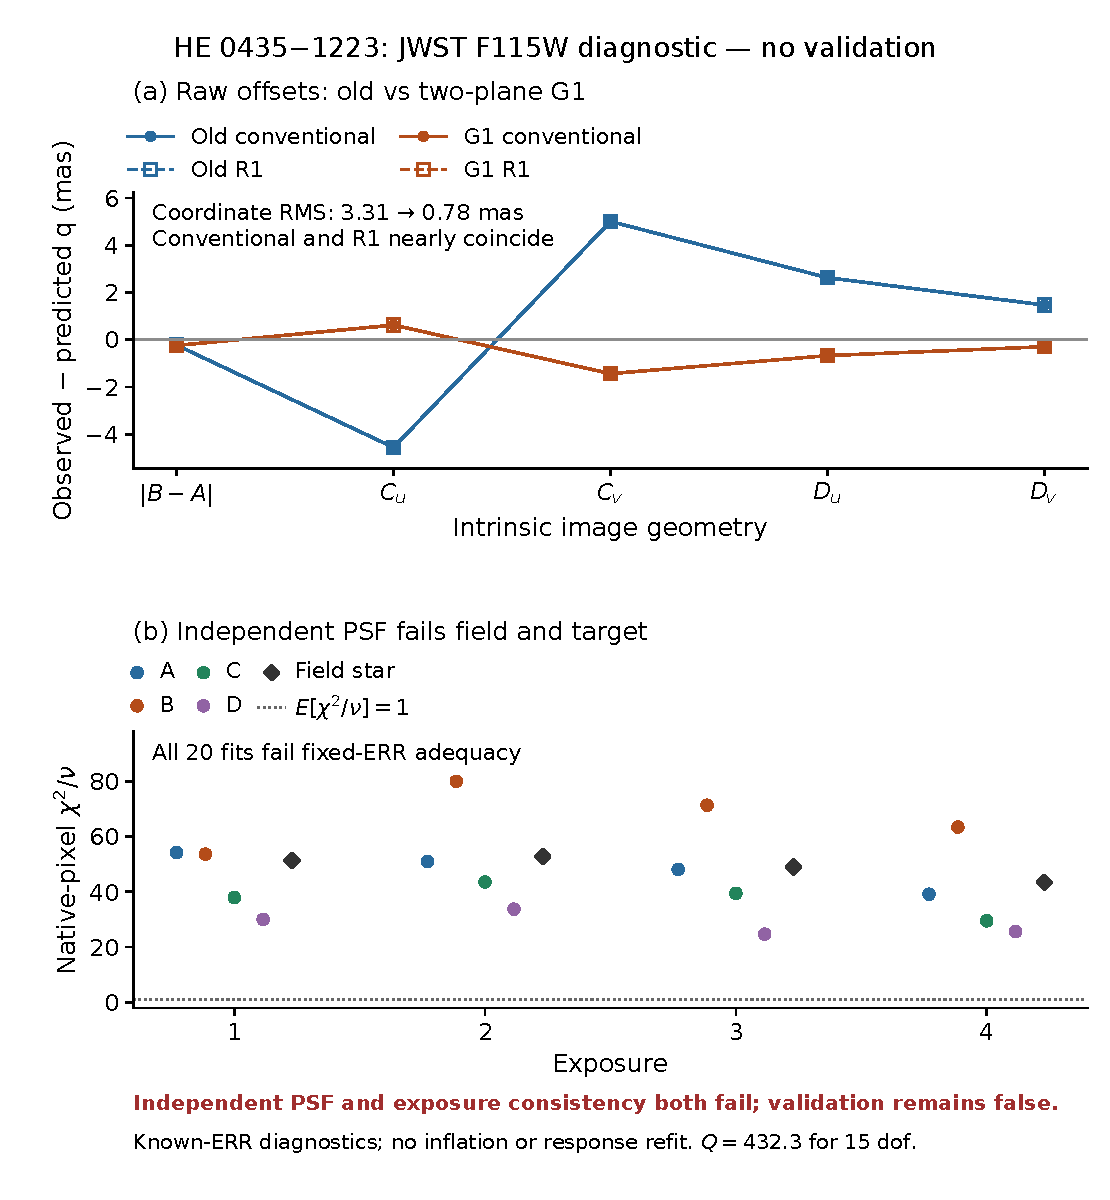
\includegraphics[width=\linewidth]{figures/he0435_jwst_geometry_diagnostic.pdf}
\caption{Unused-photon geometry diagnostic and native pixel adequacy.
Fixed G1 predictions reduce the raw geometry residuals. The severe
pixel residuals independently prevent validation; formal centroid
errors are not inflated. Conventional and R1 curves nearly coincide.}
\label{fig:he0435-jwst-diagnostic}
\end{figure}
